%%%%%%%%%%%%%%%%%%%%%%%%%%%%%%%%%%%%%%%%%
% Short Sectioned Assignment
% LaTeX Template
% Version 1.0 (5/5/12)
%
% This template has been downloaded from:
% http://www.LaTeXTemplates.com
%
% Original author:
% Frits Wenneker (http://www.howtotex.com)
% License:
% CC BY-NC-SA 3.0 (http://creativecommons.org/licenses/by-nc-sa/3.0/)
%
%%%%%%%%%%%%%%%%%%%%%%%%%%%%%%%%%%%%%%%%%

%----------------------------------------------------------------------------------------
%	PACKAGES AND OTHER DOCUMENT CONFIGURATIONS
%----------------------------------------------------------------------------------------

%\documentclass[paper=a4, fontsize=10pt, font=arial]{scrartcl} % A4 paper and 11pt font size
\documentclass{svproc}
%\usepackage[T1]{fontenc} % Use 8-bit encoding that has 256 glyphs
%\usepackage{fourier} % Use the Adobe Utopia font for the document - comment this line to return to the LaTeX default
\usepackage[english]{babel} % English language/hyphenation
%\usepackage{amsmath,amsfonts,amsthm} % Math packages
%\usepackage{url}
\usepackage{sectsty} % Allows customizing section commands
%\allsectionsfont{\centering \normalfont\scshape} % Make all sections centered, the default font and small caps
%\graphicspath{ {figures/} }
%\usepackage{geometry}
%\usepackage{float}
\usepackage{graphicx}
\usepackage{multicol}
\usepackage{footmisc}
%\usepackage{caption}
%\usepackage{subcaption}
\usepackage{cite}
\bibliographystyle{unsrt}
%\numberwithin{equation}{section} % Number equations within sections (i.e. 1.1, 1.2, 2.1, 2.2 instead of 1, 2, 3, 4)
%\numberwithin{figure}{section} % Number figures within sections (i.e. 1.1, 1.2, 2.1, 2.2 instead of 1, 2, 3, 4)
%\numberwithin{table}{section} % Number tables within sections (i.e. 1.1, 1.2, 2.1, 2.2 instead of 1, 2, 3, 4)
%\textheight=260cm
%\setlength\parindent{11pt} % Removes all indentation from paragraphs - comment this line for an assignment with lots of text
%\setlength{\parskip}{1em}
%----------------------------------------------------------------------------------------
%	TITLE SECTION
%----------------------------------------------------------------------------------------

\newcommand{\horrule}[1]{\rule{\linewidth}{#1}} % Create horizontal rule command with 1 argument of height

\title{A Comparison of Time Domain Numerical Methods for Faster Acoustic Modelling} % The assignment title
\titlerunning{Time Domain Methods for Faster Acoustic Modelling}
\author{Simon Durbridge} % Your name
\authorrunning{S.Durbridge}
%\date{\normalsize\today} % Today's date or a custom date
\institute{Dept. Engineering, Mathematics \&\ Computing\\ University of Derby\\
\email{s.durbridge1@unimail.derby.ac.uk} % optional, same for URL of homepage
} % end of address field

\begin{document}

\maketitle % Print the title

%----------------------------------------------------------------------------------------
%	Abstract
%----------------------------------------------------------------------------------------

\begin{abstract}
Interest in acoustic modelling continues to increase due to a rise in commercial demand and improvements in tool quality. Wave based modelling methods promise many benefits over the commonly used ray based methods, but the use of these methods remains restricted due to the inherent high resource demands that non-specialist computing platforms struggle to cater for. For real-time applications time domain wave solving may be of particular use, due to the inherent nature and accuracy of the solving i.e. the ability to provide direct solutions (real time audio data) as opposed to indirect solutions (impulse responses). Two potential methods of reducing computation time may be to calculate indirect solutions through sparse finite-difference time domain Methods(S-FDTD), or to calculate direct results through pseudo-spectral time domain methods. This report aims to highlight the difference between these two methods, and the potential benefits for improved solution rate. 


\keywords{Acoustic Modelling, Numerical Methods, Time Domain, Fast}
\end{abstract}


%\newpage

%----------------------------------------------------------------------------------------
%	Contents
%----------------------------------------------------------------------------------------

\tableofcontents

%\newpage

%----------------------------------------------------------------------------------------
%	Figures
%----------------------------------------------------------------------------------------

\listoffigures

%\newpage



%----------------------------------------------------------------------------------------
%	Introduction
%----------------------------------------------------------------------------------------

\section{Introduction}
Interest in acoustic modelling continues to increase due to external factors such as; A renewed focus in global standards of distributed loudspeaker system design requirements, for areas such as public address and safety(Public Address Voice Alarm(PAVA)), as well as less safety driven interests such as immersive virtual reality experiences of synthesized spaces. The benefits of improved acoustic modelling methods allows key stakeholders such as architects, acousticians, computer games and media developers, product designers and even aerospace, military and general commercial parties to leverage high quality results and create better quality products. However, time is an ever more strict constraint in many commercial development applications, and an inherent issue with high accuracy modelling is a significant increase in work-flow time as well as computational resources and specialist knowledge.\par 

A continually sought outcome of further research into numerical methods for acoustic modelling, is a reduction computation time. Is it possible to further reduce computation time for arbitrarily size problems?\par

A reduction in computation time of very large problems e.g. stadium PAVA and loudspeaker system design, will allow designers to experiment and confirm designs to both a higher degree of accuracy and with greater efficiency. Further to this, real time solving for large models could allow system technicians to monitor and adjust system performance 'on-the-fly' with greater precision. A reduction in computation time for less complex models could allow for higher quality acoustic simulations in video-games and virtual reality media. Both of the previously noted applications would benefit not only from real-time solutions from a quality perspective, but would also potentially benefit from  methods that require less memory access and/or computational resources i.e. implicit methods and general purpose graphical processing units(GPGPU). 


\par

\begin{figure}
\centering
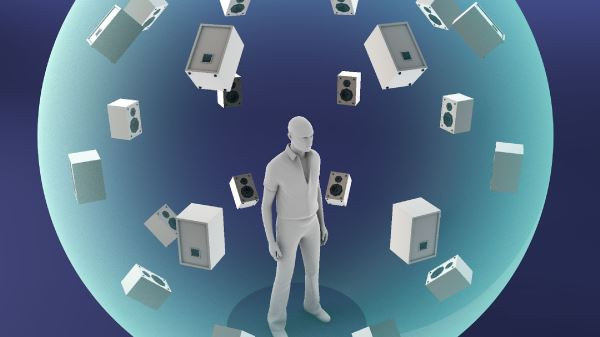
\includegraphics[width=0.6\textwidth]{googlevirtualsoundsources.jpg}
\centering
\caption{A visualisation of virtual sound sources ~\cite{googlevr2016}}
\end{figure}

%\newpage

%------------------------------------------------
\section{Acoustic Modelling}
\subsection{Applications}

\subsection{Ray Methods}

Research into spatial audio for VR may have flourished in recent past, but the foundation of localization theory remains based on the concepts explored by Rayleigh in 1907~\cite{Blauert1997}. Continued research into the field has matured and evolved understanding of these concepts, and for an in-depth review of auditory localization please review Blauert~\cite{Blauert1997}. Localization is the term given to the human capacity to binaurally (with two ears) localize sounds, laterally in the plane of the ears and in the median plane (up and down). A sources perceived location is determined by interaural time differences (ITD), phase differences, interaural level differences(ILD), and the physical listening apparatus itself (pinnae, head shape, torso, head tilting etc).

%\centering
%\includegraphics[width=0.4\textwidth]{itdexample.jpg}
%\centering
%\caption{A basic model diagram of the ITD from a source to a listener given by $\frac{r(\theta + sin \theta)}{\textit{c}}$ ~\cite{rumsey2012spatial}}
%\end{figure} 



\subsection{Wave Methods}

Many of the recent VR systems consist of a viewing headset that may be powered by a mobile phone, a games console or a computer. The headsets viewing system provides a stereoscopic vision of a 3d environment that is linked to a head tracking interface, allowing the user to explore the 'immersive' visual environment in 3d. For many of the new virtual reality platforms, ambisonics has become the signal format of choice~\cite{googlevr2016}. This choice may be due to the flexability of a system that can encode and decode arbitrary numbers of input and output channels, while inherently maintaining the spatial nature of the content.
Another benefit may be the compatability of ambisonics with concepts such as object based audio~\cite{Pike2016}. For a review of various 'spatial' audio system formats, please refer to~\cite{Wiggins2004}. Many of the newer VR platforms rely on headphones as the preferred audio system format. This may be in part due to the difficulty in producing HRTFs for multiple listeners over loudspeaker, though research in this area is continually improving~\cite{Galvez2016}. Another benefit of the use of headphones is that head tracking can be applied to HRTFs to improve the spatial audio quality~\cite{Inanaga1995} in a relatively discrete package.\\

%\begin{figure}[H]
%\centering
%\includegraphics[width=0.3\textwidth]{ambisonicmicpatterns.jpg}
%\centering
%\caption{A plot of four ambisonic microphone polar patterns (for B format)~\cite{Wiggins2004}}
%\end{figure}


%\newpage
%------------------------------------------------
\section{Time Domain Methods}
%---------------------------------------------
\subsection{FDTD}

The reverberant sound field is the steady-state of diffusely scattered sound energy in a space due to the reflection of that energy from boundaries to a high order. 
Specifically, the amplitude of these reflections are such as to balance in amplitude with the steady state (source - decay) of the acoustic system, at or beyond the critical distance from a source (a classic analogy is given by Everest)~\cite{Everest2009}. 

%\begin{figure}[H]
%\centering
%\begin{subfigure}[b]{0.4\textwidth}
%\includegraphics[width=\textwidth]{revertimedefinition.jpg}
%\centering
%\caption{An example graph of reverberation decay time $RT_{60}$}
%\end{subfigure}
%~
%\begin{subfigure}[b]{0.4\textwidth}
%\includegraphics[width=\textwidth]{clarityscore.jpg}
%\centering
%\caption{An example of the calculation of Clatiry score}
%\end{subfigure}
%\caption{Graphics pertaining to quantification of reverberant sound ~\cite{rossing2007springer}}
%\end{figure}
%\newpage

\subsection{S-FDTD}

\begin{center}
$L_T = L_W + 10 log \left( \frac{QMe}{4\pi D_{x}^2} + \frac{4N}{S \overline{a} M a}\right) + K $\\
\end{center}
where:
\begin{enumerate}
\item $L_T =$ total sound pressure
\item $L_W =$ sound power level of source
\item $\frac{QMe}{4\pi D_{x}^2}$ is a description of the sound source direct radiation properties
\item $\frac{4N}{S \overline{a} M a}$ is a description of the reverberant field properties
\item $K = \frac{\rho \textit{c}}{400}$ relating to the transfer of sound through air
\end{enumerate}

%\newpage

\subsection{PSTD}
There is a plethora of research and understanding of the objective quantification of reverberation~\cite{rossing2007springer}, less so about the subjective effects~\cite{Karjalainen2001} beyond the seminal studies of early reflections by early pioneers (even before Haas)~\cite{Haas1972}~\cite{Begault1995}. 
It may be argued that many facets of human auditory perception relate in some way to the perception of reverberation. The concepts of interest in this paper are those linked with localization and perception of the auditory scene. Within these concepts are Haas/Precedence effect, and auditory masking.

%\begin{figure}[H]
%\centering
%\includegraphics[width=0.4\textwidth]{coreydiagram.jpg}
%\caption{A diagram of the layout for Corey's listening test\cite{Corey2002}}
%\end{figure}

%\newpage
\subsection{Reverberation Algorithms}
\subsubsection{filter based reverb}

A relatively simple electronic method of simulating reverberation is that derived by a feedback loop. An analogy of this system is that of a tape deck with a looped reel of tape~\cite{Begault1995}. A delay presented between the read and write heads of the tape deck, with the write head writing not only new signals to the tape but an attenuated version of the signal read by the read head producing a decaying echo. In the frequency domain, such a system presents a comb filtered response as a version of a signal is interfering with itself but staggered in time.\\ 
When a series of these reverberation filters are cascaded together with varying delay times, it is possible to create a slightly metallic sounding reverb~\cite{Begault1995}. An improvement to this method is to add a single pole low pass filter to the delay block for simulating attenuation, and to add  a number of all-pass filters in series after the delays have been summed in order to reduce periodicity of the delay signal~\cite{Logan1961}.\\

%\begin{figure}[H]
%\centering
%\includegraphics[width=0.4\textwidth]{apfblockdiagram.jpg}
%\caption{A block diagram of a Schroeder and Logan all pass filter\cite{Begault1995}}
%\end{figure}

A third method of creating a reverb effect is to convolve a signal with the IR of the system to be emulated~\cite{Lee2010}, or with a decaying 'shaped' noise function~\cite{Lien2016}. This process in discrete digital systems involves multiplying a current sample and $n-1$ previous samples with $n$ coefficients, thus adding varying amounts of the previous portion of the signal to the 'current' sample. This method is also required for digitally applying the measured IR of a real space to some audio for simulation purposes, and the same again for a modelled or calculated IR using one of the modelling techniques discussed below. 

\subsubsection{modelling}
Geometric based modelling methods are those based on assumptions of plane wave propagation and ray based geometry to calculate the time of flight and  of some sound between a source and a receiver. These methods include image source modelling, ray tracing, cone tracing and variations~\cite{Elorza2005}. Geometric modelling can be used for creating IRs suitable for auralization~\cite{Oxnard2012}. This report will focus on the previously mentioned image source technique.\\

The image source(IMS) technique uses a rectilinear geometry with some basic frequency-independent absorption characteristic, and conceptually multiplies that geometry in symmetric fashion around the origin geometry~\cite{Allen1979}. The effective time of flight and number of virtual boundaries passed indicates some absorption, reflection order and time delay between the source and receiver. Thus, the IR of the geometry can be calculated with accuracy up to the order of the simulation i.e. how many times the geometry is mirrored. This method cannot handle an irregularly (not piecewise linear~\cite{Borish1984}) shaped geometry, any obstacles, and assumes that the ray represents part of a plane wave whose wavelength is much smaller than any part of the geometry~\cite{Elorza2005}. This method is however relatively simple, fast to compute and is potentially a good method for calculating arrival times and amplitudes of early reflections for a binaural pair of receivers down to the rooms Schroeder frequency.

%\begin{figure}[H]
%\centering
%\includegraphics[width=0.4\textwidth]{imagesourcediagram.jpg}
%\caption{A diagram of a cascaded geometry in the IMS method\cite{Hill2012}}
%\end{figure}

Using the calculated reverb decay time $RT_{60}$ to set up an IIR reverb and the early reflection results from an IMS simulation~\cite{Oxnard2012}, it is potentially possible to combine the two responses to create and artificial reverberation for VR environments that provides early reflections for localization, but is not to such a high order as to become computationally expensive~\cite{Lee2010}. \\

Wave based modelling methods directly model spaces by calculating solutions to a discretized partial differential equation across the geometry~\cite{Botteldooren1995}~\cite{Bilbao2013}. For linear and room acoustics, the equation used is often the linearised Navier-Stokes or Euler diffusion style equations that satisfy the conservation laws. Depending on the solving scheme used, the geometry will need to be discretized to at least 2 points per wavelength (in line with Nyquist theorem) and potentially beyond 10 points\footnote{particularly for explicit finite different and finite element methods} per wavelength to satisfy the Courant condition~\cite{Siltanen2013}. The result is that problems become exponentially large and thus expensive to solve up to high frequencies. However, some methods such as the PTSD have been used to calculate up to low-mid frequencies in real time~\cite{Angus2010}~\cite{Savioja2010} and may in future become suitable to calculating low frequency portions of hybrid models in VR~\cite{Southern2012}.

%----------------------------------------------------------------------------------------
\newpage
\section{Experiment Protocol}
\subsection{experiment aims}


\subsection{experiment method}
Users will be asked to evaluate 3 different listening environments, with two stimuli, of two people talking in the space and a stereo pop music track respectively. The test results will be analysed for localization error, front-back reversals. There will be five potential reverb scenarios to evaluate in each environment: 
\begin{itemize}
\item convolving with an IR of a real space
\item a derived reverb with no early reflections 
\item a low order image source IR combined with a derived reverb
\item a high order image source IR
\item a control instance of the signals without spatial reverb
\end{itemize}


\section{Conclusion}
The intention of this paper was to explore some of the key psychoacoustic and physical principals behind the localization of sounds in relation VR, so that a listening test may be designed for evaluating the effect of different reverb synthesis methods on localization in VR applications. Key texts by Begault~\cite{Begault1995} , Wiggins~\cite{Wiggins2004}, Blauert~\cite{Blauert1997} and Rumsey~\cite{rumsey2012spatial} denote the importance of reverb in the context of localization and perception with relation to spatial audio.



%----------------------------------------------------------------------------------------
\newpage
\section{References}

\bibliography{myLibrary}{}
\bibliographystyle{plain}

\end{document}